\documentclass[a4paper]{article}

\usepackage[margin=1in]{geometry}
\usepackage{CJK}
\usepackage{graphicx}

\title{Report for EI339 Artificial Intelligence: Homework 3}
\author{517030910384 徐尚宁}
\date{}

\begin{document}

\begin{CJK}{UTF8}{gbsn}
    \maketitle
\end{CJK}

\section*{Q1}

Values of $V_\textrm{opt}$ after each iteration are given in the following table:

\begin{table}[h]
    \begin{tabular}{|l|l|l|l|l|l|}
    \hline
    Iterations\textbackslash States & -2 & -1 & 0 & 1 & 2 \\ \hline
    0 & 0 & 0 & 0 & 0 & 0 \\ \hline
    1 & 0 & 16 & 0 & 70 & 0 \\ \hline
    2 & 0 & 16 & 49 & 70 & 0 \\ \hline
    \end{tabular}
\end{table}

\section*{Q2}

We implement and visualize the SARSA algorithm with the $\epsilon$-greedy policy
in \texttt{cliffwalk.py}. Figure~\ref{fig:an-execution-of-sarsa-algorithm} shows
the Q-values and the optimal policy from an execution of our implementation. For
brevity, we do not include the full matrix for the Q-values.

\begin{figure}[ht]
    \centering
    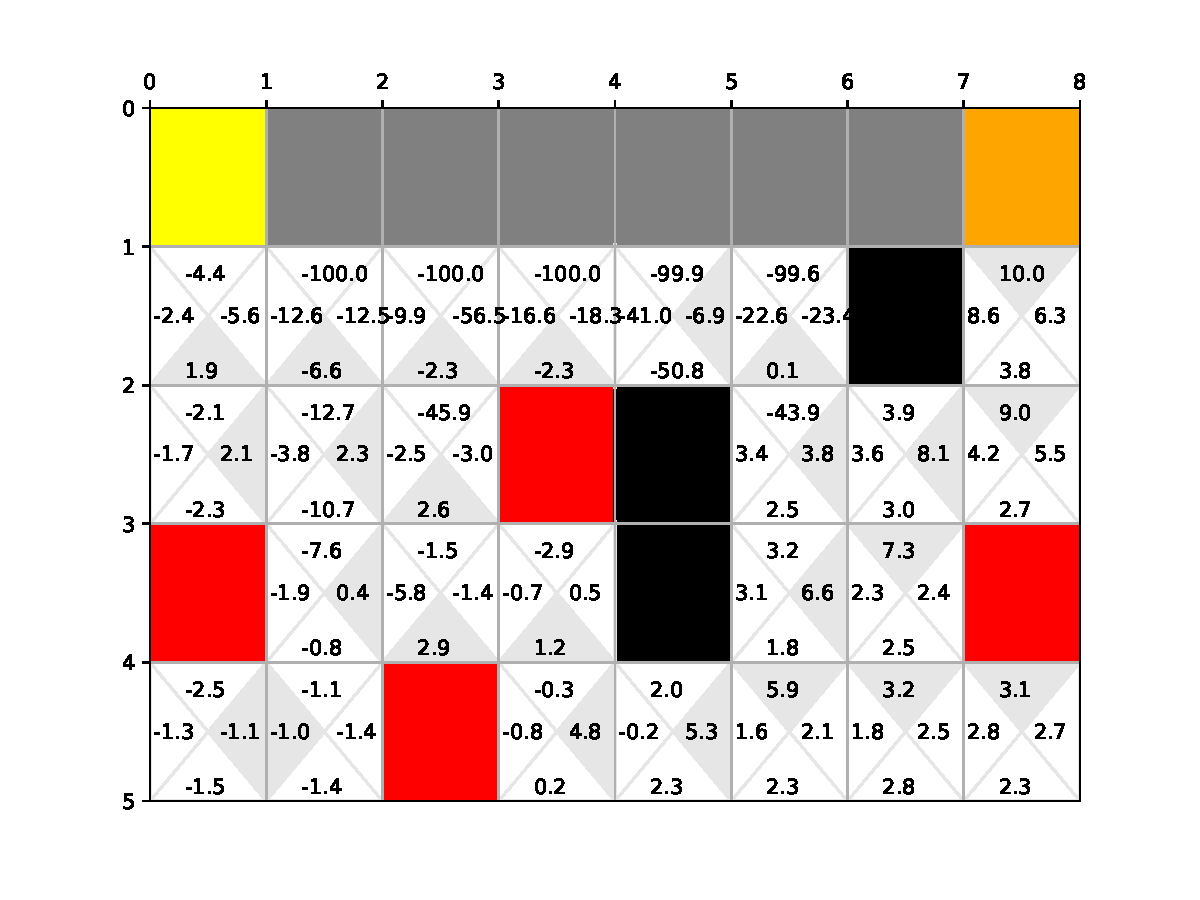
\includegraphics[width=\linewidth]{q_values_and_policy.pdf}
    \caption{Visualized Q-values and the optimal policy (optimal action shaded
    for each state) in a run of our implementation of SARSA. $500, 500, 100$
    episodes for $\epsilon = 1, 0.5, 0$, respectively. The policy and Q-values
    for the yellow and the red squares are not displayed.}
    \label{fig:an-execution-of-sarsa-algorithm}
\end{figure}

The implementation strictly conforms to the SARSA algorithm and the
$\epsilon$-greedy policy, so we choose to discuss one outstanding issue with our
implementation and the problem setting, namely the existence of circles and
self-loops in the all-exploitation strategy.

After computing the Q-values with $\epsilon = 1$ and 0.5, there may exist a
cycle consisting of states and actions or a self-loop consisting of a state and
an action that keeps hitting the obstacle. In our implementation, if an agent at
state $s$ takes the optimal action $a$ and hits a wall, its position won't
change and its next action is still $a$ (since $a$ is optimal), resulting in a
transition of $(s, a, 0, s, a)$, but its Q-value is still updated. Setting $r =
0, s' = s$ and $a' = a$ in the assignment of $Q_\pi$, we obtain
\[
    \hat Q_\pi(s,a) \gets (1 - \eta + \eta\gamma) \hat Q_\pi(s,a)
\]
What if all Q-values at $s$ is negative? The agent is actually ``rewarded'' for
hitting a wall because $\hat{Q}_\pi(s, a)$ is discounted by $1 - \eta +
\eta\gamma$ and becomes larger. The case for a cycle is similar to the case for
self-loops.

The main reason for this behavior lies in the assignment of rewards in the
problem setting. The combination of high penalty for falling off cliffs and low
rewards for the end state discourages the agent from moving towards the end
state, as evident in a large number of negative Q-values. Just imagine that you
are going to somewhere entirely unfamiliar to you to collect some super tasty
mushrooms (orange square) under the risk of being arrested. Tripping over stones
(red square) doesn't seem like a big deal, and you should probably just stay at
home or linger around some proven safe areas (like hitting a wall), because the
reward doesn't justify the risk.

The end result is that sometimes the program will be stuck in cycles and loops
and not exit successfully.

\end{document}
